\section{Introduction}
\label{intro}

%{\bf OUTLINE}
%
%\begin{enumerate}
%
%%\item The background of image search and image clustering
%%(cite some related work in this space here). Basically there are three
%%kinds: (1) using contextual info (2) using visual attributes and (3) both.
%%What's the state of the art technique and result? Show some example (figs).
%%
%%\item  What are the challenges in image search: (1) right context (2) context
%%representation (bag of words, bag of concepts, topics, etc.) (3) clustering
%%algo (4) presentation (diversification?) (5) performance
%%(incremental, caching).
%%
%%\item What are the problems in existing solutions.
%%
%%\item Briefly describe our approach, why it works, and summarize our results.
%\item Motivation: traditional image search is by relevance only and ignore
%the semantics of the image and doesn't disambiguate images of different
%entities. As a result, search results can be either highly ``mixed'', or
%highly ``uniform'' and missing the diversity. (Give a screen shot of google
%image here.)
%\item What do we want to do? A succinct problem statement here.
%\item Existing techniques:
%\begin{enumerate}
%\item visual based -- visual features and machine learning:
%visual similarity have low precision, needs labeling, and what else??
%\item context based -- bag of words: bag of words can't adequately capture
%the meaning of context; contexts are not easy to define.
%3) hybrid approach: the gap between the visual semantics and the text
%semantics; slow!
%\end{enumerate}
%Give some concrete examples for each of these cases to illustrate why
%they don't work or insufficient.
%%\item Getting signals from images themselves are difficult so context of images
%%can be used to identify and cluster images
%%\item Bag-of-word based contexts are insufficient
%%\item Concept-based contexts carries better semantics
%%\item Clustering is hard because the relateness among sub-clusters may not be
%%obvious: a special similarity method has to be used
%%\item Incremental cluster helps to scale
%\item Our approach:
%\begin{enumerate}
%\item it's a flexible framework that can incorporate both text and visual
%signals, but with emphasis on text (reason is text sigals are easier to
%pick up and more explicit);
%\item use conceptualization by wiki concepts to better understand the concept
%before clustering them;
%\item provide a topic for each cluster
%\item tripple clustering algo to improve both purity and inverse purity;
%\item online and offline division to make it much much faster,
%and practical for image search!
%\end{enumerate}
%
%\item Key contributions of this paper:
%\begin{enumerate}
%\item design and implement a framework of clustering images by
%context conceptualization outperforms peers by significant margins in
%terms of f-measure;
%
%\item online-offline split make the framework feasible for web search
%(1 sec response time!)
%
%\item extensive comparisons to show that our algo outperforms peers.
%\end{enumerate}
%\end{enumerate}

%Here is the general introduction to our project.
%
%We are dealing with the search result of Google Image search engine. We catch the original webpage of each search result item, and then extract the context of each webpage with given keyword. At last, we extract the semantic information for contexts and do cluster on the search result.
Images are one of the most abundant multimedia resources on the Web.
Most commercial search engines offer image search today,
which enables the user to retrieve images by a search term.
%Along with the development of image searching techniques,
%one can easily retrieve concerned images by specifying a keyword.
By default, all existing image search engines rank the returned images
by the relevance of their contexts (i.e. the web pages they are
embedded in) to the query keyword. \figref{fig:search-bean-on-google}
shows the result of the search for ``bean'' on
\textit{Google Image}\cite{google}.
The result appears to be a random mix of many different entities related
to the keyword ``bean'', e.g.,
``Mr. Bean (comedian)'', ``Sean Bean (actor)'',
``beans (crop)'', etc. Ambiguous search terms like this
are not rare: Google Image returns at least two different entities for
``kiwi'', three for ``explorer'', %six for ``Anderson''
and over ten different persons named ``Jerry Hobbs''!

\begin{figure}[th]
\begin{minipage}[t]{\linewidth}
	%\centerline{\psfig{figure=screen_bean3.eps,width=\columnwidth}}
\centering
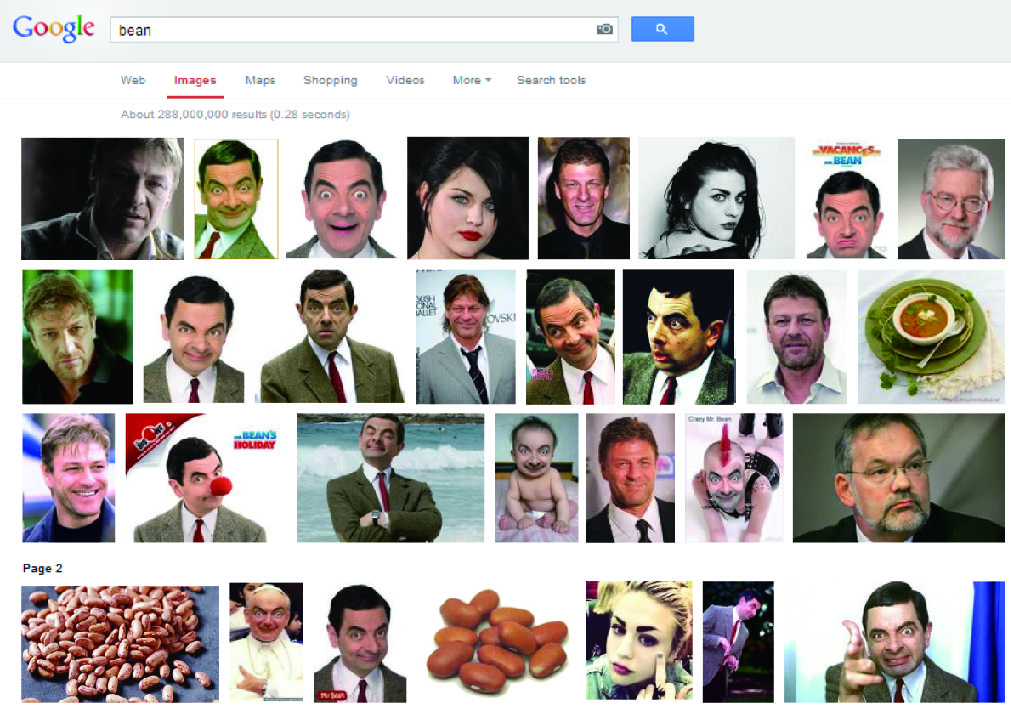
\includegraphics[width=\columnwidth,natwidth=1011,natheight=708]{screen_bean3.jpg}
	\caption{Search Result of ``bean'' on Google Image}
	\label{fig:search-bean-on-google}
\end{minipage}
\begin{minipage}[t]{\linewidth}
	%\centerline{\psfig{figure=screen_bean_subj.eps,width=\columnwidth}}
\centering
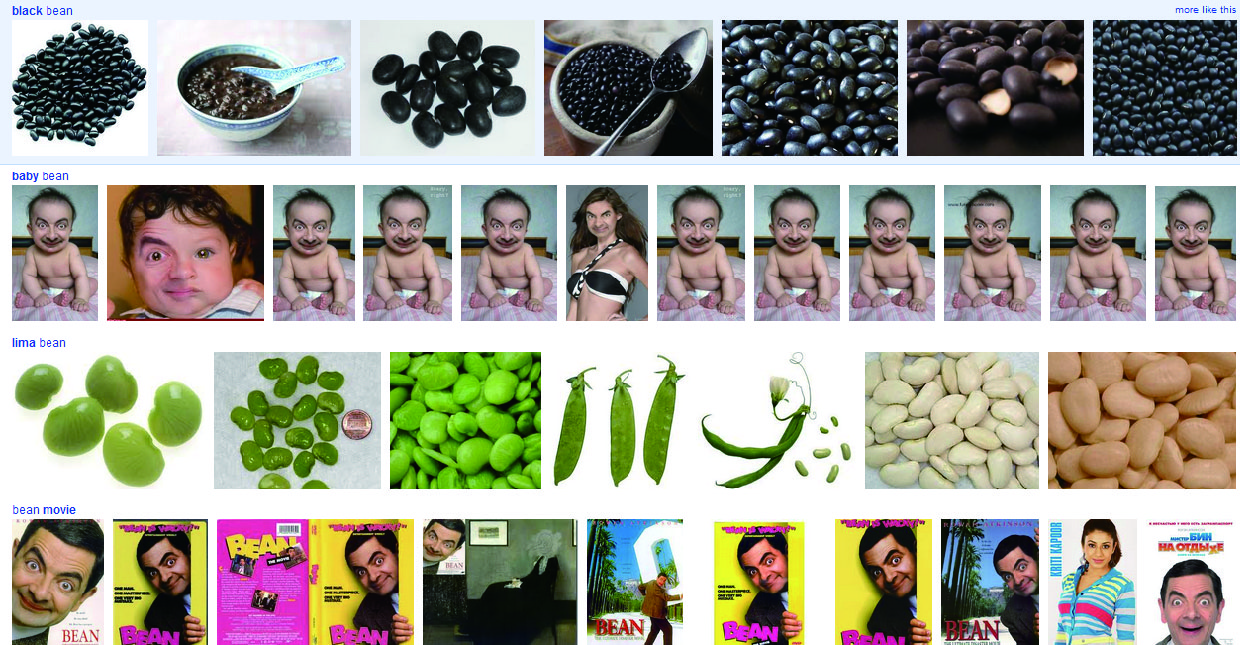
\includegraphics[width=\columnwidth,natwidth=1240,natheight=645]{screen_bean_subj.jpg}
	\caption{Search Result of ``bean'' grouped by subject on Google}
	\label{fig:search-bean-by-subj}
\end{minipage}
\vspace*{-3mm}
\end{figure}

Some search engines attempt to improve the user experience by introducing
an ``order by'' feature where images can be sorted by color, size, type
or subject. Among these, order-by-subject provided by Google
(in \figref{fig:search-bean-by-subj}) comes closest to distinguishing
images by their semantic content.
%They achieve this by computing the top $k$
%queries containing the search term (e.g., ``black bean'', ``baby bean'' and
%``bean movie'') that would produce the best results according to a search log.
%Then the top results from these $k$ modified queries are presented
%grouped by the $k$ subjects.
%This approach has the following limitations.
This system has the following limitations when showing the images to users.
First, it doesn't actually distinguish entities. For example, Mr. Bean appears
under two different subjects in \figref{fig:search-bean-by-subj}.
Second, the set of images returned with the ``order-by'' feature
is very different from the original search result because of the different
search terms.
%Third, because of the need to submit multiple queries, $k$
%cannot be large and hence limit the number of subjects and the
%diversity of the result.

%{\color{red}
%Google Image adopts a strategy to reorganize the search result by
%grouping the images in to different ``subject''s. (See \figref{fig:search-bean-by-subj})
%They obtain the subjects by ranking terms related to the
%query by making use of the search log. However, this makes two problems:
%First, the search result will be very different from the original relevance based approach.
%(Compare \figref{fig:search-bean-on-google} with \figref{fig:search-bean-by-subj}) This
%makes the search result less relevant to the query. Second, the same entity can be recognized
%as different in subject.
%}

%
%The current result delivery strategy of image search engines has
%the following problems:
%First, if the user is looking for a particular ``bean'' without knowing the
%full name, e.g., Sean Bean, it is actually not easy for her to
%navigate through the myriads of pictures to find the portraits she wants.
%%If the entity that the user is looking for is not popular, its images
%%can be ranked low and hence excluded from the first set of results.
%Second, if the user doesn't know how Sean Bean looks,
%\footnote{For the record, Sean Bean appears in the first, fifth images
%of the first row and first, forth and seventh images in the second row
%in \figref{fig:search-bean-on-google}.} then
%she has to click open every possible image to check the description on
%the web page, which is very tedious and time consuming.
%Finally, if the search term has a very dominant meaning, e.g.,
%``galaxy'', then almost all the images in top results
%are about this very concept or entity (e.g., the system of stars),
%with the images of other entities (e.g. the phone or the sports team)
%buried deep in the results. Such image search results
%are less diverse or interesting.
%

%a list of images relevant to the keyword. However, this kind
%of result is always a mixture of many kinds of entities.
%For example, if you search for ``bean'' in \textit{Google Image} \cite{google},
%you will get a list of images that are related to ``bean'' (See
% \figref{fig:search-bean-on-google}). The keyword ``bean''
%may refer to The resulting list is mixed
%with these different entities. This result is very unfriendly to
%users, since it is difficult to find out an entity from these mess results,
%e.g. ``Sean Bean''. This kind of ambiguous search queries are very
%common.

This paper is concerned with the problem of clustering web images
according to the entity or concept they represent.
Once the images are clustered, the search engine can
return {\em original} set of search results classified by distinct entities,
offering easier accessibility and more diversity.
%current search engines described above. We reorganize the search results
%and divide them into several semantic clusters. Within each cluster, the images
%are about the same entity.

In the past, there has been numerous research efforts on image clustering. These
efforts can be roughly divided into three categories: visual-based,
context-based and hybrid approaches.

Visual-based methods
only take the visual features, such as SIFT descriptors,
edge histogram, color, contrast, into account \cite{Fu2011, ZhongLL11},
and these are often insufficient in distinguishing real entities.
For example, some images of {\em Mr. Bean}
in \figref{fig:search-bean-on-google} are very different by the look,
while other images of {\em Mr. Bean} {\em Sean Bean} are fairly
similar as they both wear suits.
%On the other hand, high level visual recognition
%techniques are not powerful enough yet to accurately identify images at entity
%or object level. For example, state-of-the-art object annotation technique has
%a humble accuracy of 0.34\cite{Li09scene}.
On the other hand, high level visual object recognition
techniques\cite{Li09scene, Krizhevsky12} focus on detecting objects like
bottle, dog, grass, etc. in an image, but are still insufficient for
distinguishing entities. For example,
they are not able to tell the fruit apple from Apple company icon,
or tell one person from another.

%The first and obvious approach is called visual-based or
%``content-based'' approach. This kind of
%approaches only takes the visual features into account \cite{Fu2011, ZhongLL11}.
%The visual features used in these techniques are usually divided into two
%classes: local features and global features. Local features are extracted
%from the surrounding pixels for each points, such as SIFT descriptor, edge
%histogram, etc. Global features are color, brightness, contrast, gray scale,
%etc. Content-based image clustering uses local, global or hybrid of these
%features to construct vector representation of the images and then evaluates
%the similarity among these vector representations.
%The problem with content-based image clustering
%is that the visual effects of the same entity may be diverse while different
%entities may share similar visual cues. For example, some images of ``Mr. Bean''
%in \figref{fig:search-bean-on-google} are very different by the look.
%The fourth one in the third row is more like a baby while
%the second one in the last row is similar to the Pope!
%However, when you look at the some of images in the second row,
%``Mr. Bean'' is visually similar to ``Sean Bean'',
%since they are both in suits. For these reasons, low level
%visual features are usually inadequate for understanding of
%the meaning of the images.
%On the other hand, existing high level visual recognition
%techniques are not powerful enough to accurately identify images at entity
%or object level. For example, state-of-the-art object annotation technique has
%a humble accuracy of 0.34 \cite{Li09scene}.

Context-based image clustering methods use only
textual information in the context of the image.
The textual information refers to URL, descriptive tags for the image,
the surrounding text and even search result snippets \cite{Jing2006}.
%With these contextual signals, a bag-of-words vector space model can be built
%to capture the pairwise similarity of the images. Methods in this approach
%often follow two main steps: identifying a meaningful context
%and representing the context.
%To identify the context, most of the existing
%work uses text within a limited window around the image or
%extracted visual blocks that contains the image \cite{VIPS}.
To represent the context, all previous work use bag-of-words or
n-grams model \cite{Jing2006}.
The bag-of-words model can not capture the semantics of the context
in an accurate way for three reasons.
First, limited length of context provide insufficient signals
in words model. Second, often phrases are more
reasonable and accurate semantic unit than words.
For example, bag-of-words model divides the term ``Research in Motion''
into ``research'' and ``motion'', which destroys the original meaning.
Finally, natural language is ambiguous. ``apple'' may refer
to an IT company or a kind of fruit.
Bag-of-words model treats every ``apple'' term
equally.
%so that text which talks about ``Apple Inc.'' and text about
%``apple fruit'' are more similar than the truth.
Similar arguments hold for n-gram models.

Hybrid approaches combine the visual features
with textual features.
%Some researchers tried to achieve this combination by
%producing a similarity score from the weighted sum of these two types
%of features \cite{LeukenPOZ09}.
%However, visual features are quite different from textual ones,
%and there's no explicit relation between them, hence no good ways of
%determining the weights.
The semantic gap between the visual and textual features
makes it difficult to directly combine them into one uniform similarity measure.
For this reason, some hybrid algorithms resort to co-clustering on
visual and text simultaneously such as MMCP \cite{Fu2011}.
But such approach is iterative, time consuming and
thus not suitable for online applications such as image search.

In this paper, we propose a new context-based approach that
%can incorporate both
%textual and visual signals. Different from the previous hybrid approaches,
%we
emphasizes on textual signal understanding.
%and use visual signals
%as {\em complements} when there is insufficient textual signals.
The reason to focus on text is that, we believe, unlike visual signals,
textual signals from the right context explicitly reveal
the semantics of the image.
%%The key is of course to get the correct context.
Our approach is different from the existing context-based image clustering
in three aspects. First, we explicitly disambiguate the context text
by converting each phrase to an unambiguous concept from an
external knowledge source. We call this process ``conceptualization''.
In this paper, we use
Wikipedia \cite{wikipedia} as our knowledge source,
and conceptualize the phrases by linking the phrases to
Wikipedia concepts/articles. Conceptualization has been previously shown
to be a better way to understand
textual signals than bag-of-words model.\cite{Song11:Conceptualize}
%,WangWWZ12:tables,WangLWZ12:topic}.
Second, our method provides concept labels to annotate
each cluster of images by accumulating the concepts in the contexts
from the clusters.
With these labels, users can conveniently grasp what each
cluster is about. Third, we propose a modified version of
hierarchical agglomerative clustering (HAC), which is more robust to noise
and apply it to a tri-stage clustering framework.
The tri-stage clustering can guarantee the purity of each cluster while
improving the inverse purity, i.e. forming as large clusters as possible.
The experimental result shows that our approach significantly outperforms
competiting algorithms, and reaches very high purity, F-measure and
NMI scores.

Furthermore, we separate the system into online and offline
components to be more practical in a search engine.
Offline component turns source pages of the images into lists of
concepts. Online component extracts the image and query contexts (in terms of
concepts) and clusters the contexts.
%Query context is the text surrounding each occurrence of the query term
%in the host web page,
The extraction can be accomplished in linear time.
To minimize the response time, we cluster images incrementally, that is,
page by page, where each page has a limited number
(e.g. 100) of images. Users can click to next page to see more entities.
Such arrangement is lightweight and is
able to deliver clustering result in 1 second.
A partial result of searching for ``bean'' on our prototype image search system
is shown in \figref{fig:demo-bean}.
Every cluster shows the
most relevant images about a distinct entity, and each cluster is labeled with
the top 5 concepts. For example,
the four clusters in \figref{fig:demo-bean} have been correctly identified
as {\em Mr Bean}, {\em Sean Bean}, {\em Frances Bean Cobain} and
{\em Phaseolus vulgaris}
(the official name for ``common bean'').

\begin{figure}[th]
\centerline{\psfig{figure=proto_bean.eps,width=\columnwidth}}
\caption{Partial Search Result for ``bean'' on Prototype System}
\label{fig:demo-bean}
%\vspace*{-3mm}
\end{figure}
%need to clustering all of the images offline which is not practical and inaccurate.

In sum, this paper makes the following contributions.
%\begin{enumerate}
%\item We design and implement a framework of clustering images by
%conceptualizing their text contexts, and the framework
%outperforms the existing state-of-the-art systems by significant margins
%and achieves high accuracies
%\footnote{Web demo: \url{http://202.120.38.145:4081/}.};
%\item The framework generates representative
%concepts (i.e., semantics tags) to annotate each image cluster;
%\item The online-offline split in the architecture reduces the online
%processing time which enables feasible web image search.
%\end{enumerate}

1) We design and implement a framework of clustering images by
conceptualizing their text contexts, and the framework
outperforms the existing state-of-the-art systems by significant margins
and achieves high accuracy
\footnote{Web demo: \url{http://202.120.38.145:4081/}.};

2) The framework generates representative
concepts (i.e., semantics tags) to annotate each image cluster;

3) The online-offline split in the architecture reduces the online
processing time which enables feasible web image search.

The rest of the paper is organized as follow.
\secref{sec:algo} presents the structure and each component of our
framework;
%\secref{sec:implement} discusses some implementation
%details and optimizations;
\secref{sec:eval} demonstrates the experimental results;
\secref{sec:related} introduces some related work while
\secref{sec:conclude} concludes the paper.

